\documentclass[a4paper, 11pt, landscape]{article}
\usepackage[landscape, left=2cm, right=2cm, top=2cm, bottom=2cm]{geometry}
\usepackage{multicol}
\usepackage{graphicx}
%\setlength\columnseprule{0.5pt}



\title{Review of Group Project}
\author{C. Funck \& M. Dittberner}
\date{Friday 10\textsuperscript{th} May, 2013}


\begin{document}

	\maketitle
	\vfill
	
	\begin{multicols}{3}
		\section{Done so far...}
			\begin{itemize}
				\itemsep 0pt
				\item Simulation procedure automatized
				\item Build a DB with simulation data
				\item {\it Toolbox} to visualize the simulation data
			\end{itemize}
		
		\vfill
		\columnbreak
		
		\section{Outlook}
			\begin{itemize}
				\itemsep 0pt
				
				\item Poster of Quantum Dot \& Solar Cell processing
				\item Documentation: Interpreting results, MATLAB
			\end{itemize}		
		
		\vfill
		\columnbreak
		
		\section{Questions}
			\begin{itemize}
				\itemsep 0pt
				\item Difference Quantum Dot \& Nanocrystal? \\
							(Semiconductor nanocrystals in the sub-10 nm size range are often referred to as quantum dots)?
				\item Simulation of other materials?
				\item What is the date of the presentation?
				\item Need more disc space.
				\item How relevant is MATLAB work, are the Simulation data?
							\begin{itemize}
								\itemsep 0pt
								\item[$\rightarrow$] Storage on a server?
								\item[$\rightarrow$] Documenting MATLAB work (User, Maintainer)?
								\item[$\rightarrow$] Installer for scripts and functions ({\it Toolbox})?
							\end{itemize}
			\end{itemize}
	\end{multicols}
		
	\newpage
	
	\section{Some Examples of the Simulation Results}
		\subsection{Quantum Dot Structure}
			\begin{figure}[htbp]
				\begin{minipage}[t]{0.48\textwidth}
						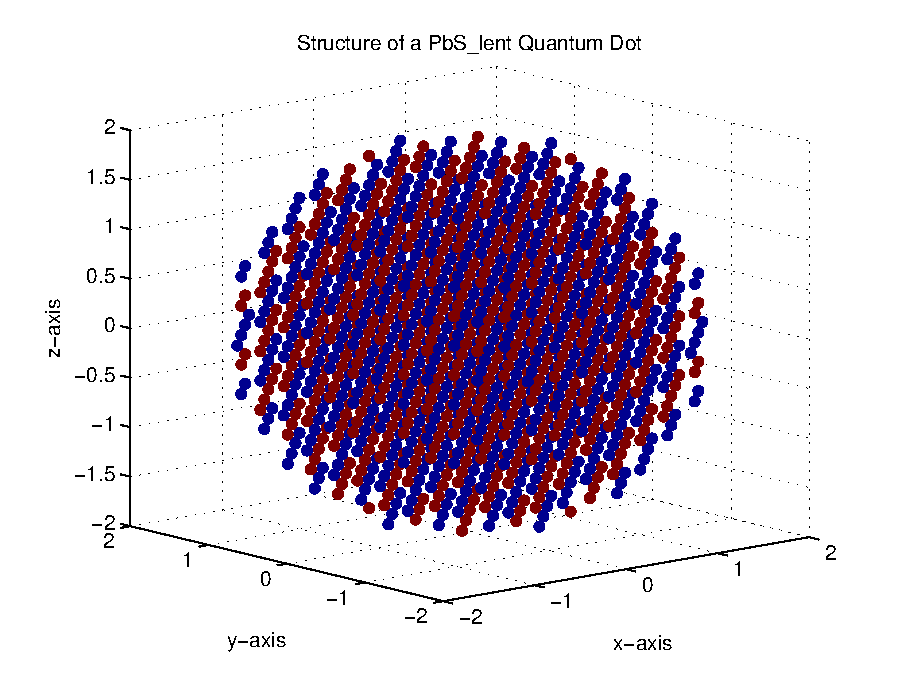
\includegraphics[width=\textwidth]{figures/StructurePlotPbS.eps}
						\caption{Atomic Structure of a PbS Quantum Dot of 4nm diameter}
				\end{minipage}
				\hfill
				\begin{minipage}[t]{0.48\textwidth}
						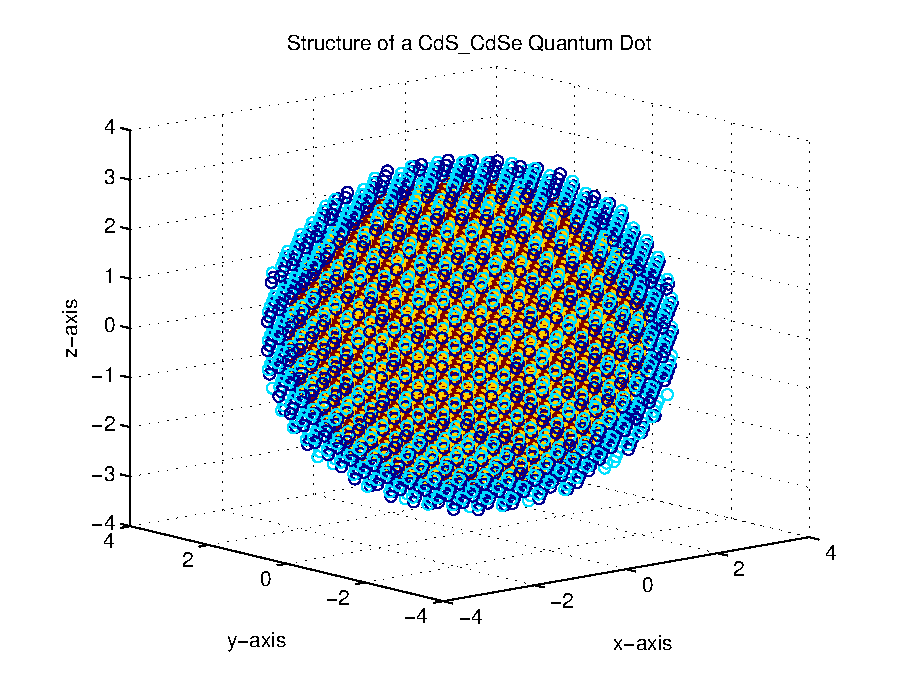
\includegraphics[width=\textwidth]{figures/StructurePlotCdS_CdSe.eps}
						\caption{Atomic Structure of a CdSe-CdS Quantum Dot with 6nm core
										 diameter (CdSe) and a 7nm shell diameter (CdS)}
				\end{minipage}
			\end{figure}
		
		\newpage
		\subsection{Wavefunctions}
		\subsubsection*{Wavefunctions of different radii}
			\begin{figure}[htbp]
				\centering
				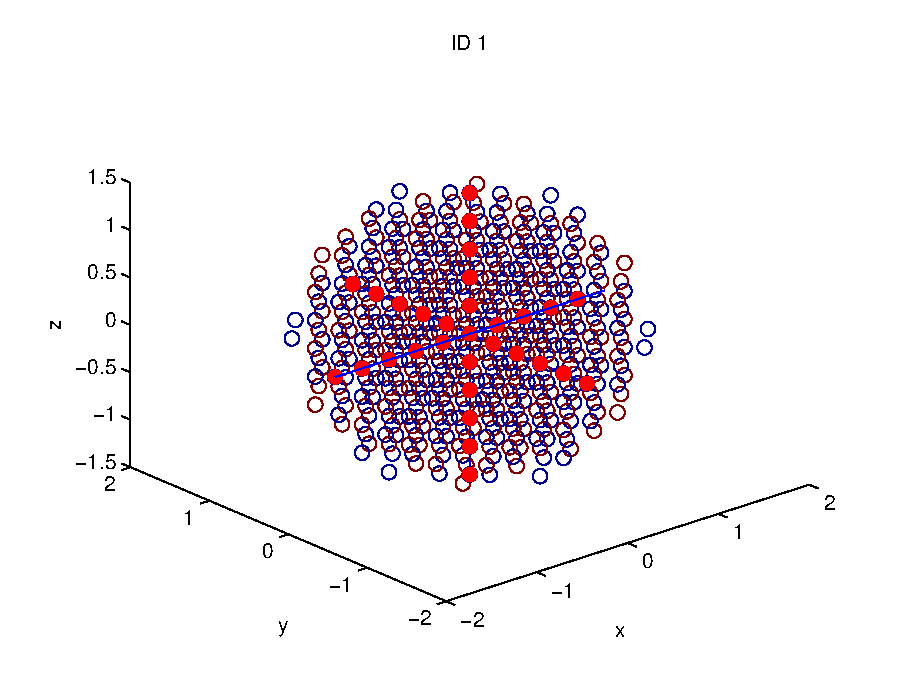
\includegraphics[width=0.6\textwidth]{figures/gridPlotAxis.eps}
				\caption{Quantum Dot structure showing axes along which wavefunctions are plotted.
								 Red dots are atoms that are taken into account for the function}
			\end{figure}
		
			\begin{figure}[htbp]
				\centering
				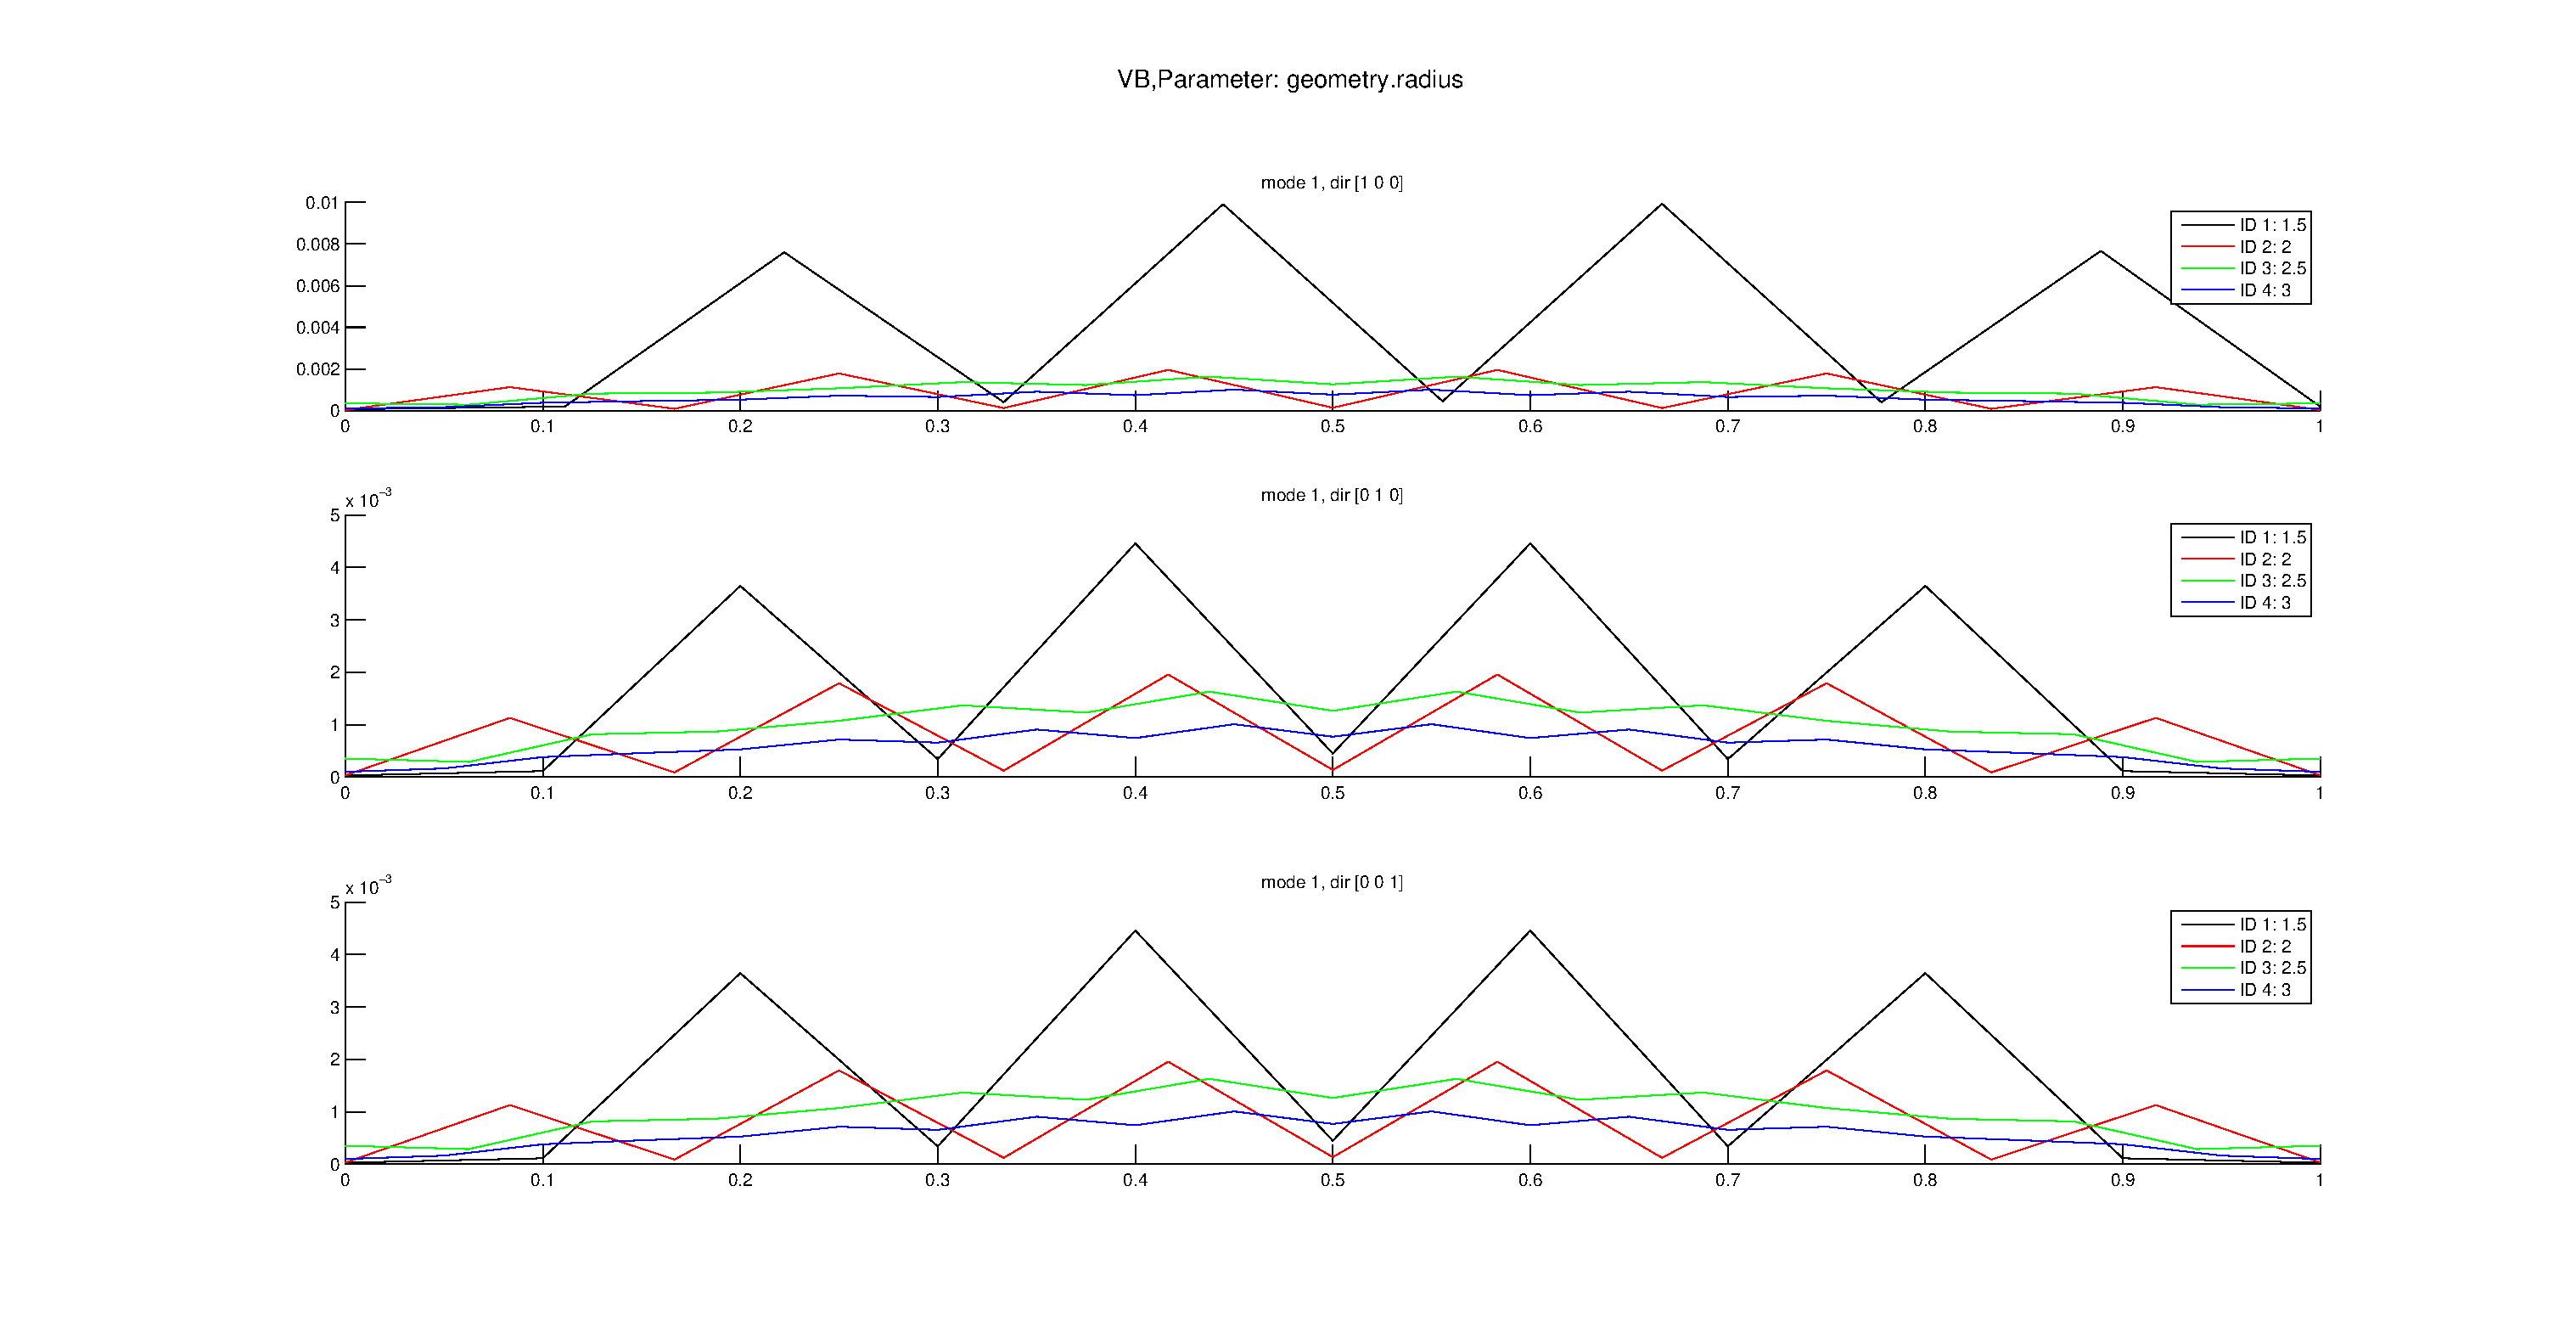
\includegraphics[width=0.9\textwidth]{figures/EVPlot3AxesMod1.eps}
				\caption{Wavefunctions for different radii and directions in the Valence Band Mode 1. The radii are {\it normalized}!}
			\end{figure}
			
			\newpage
			\begin{figure}[htbp]
			  \centering
				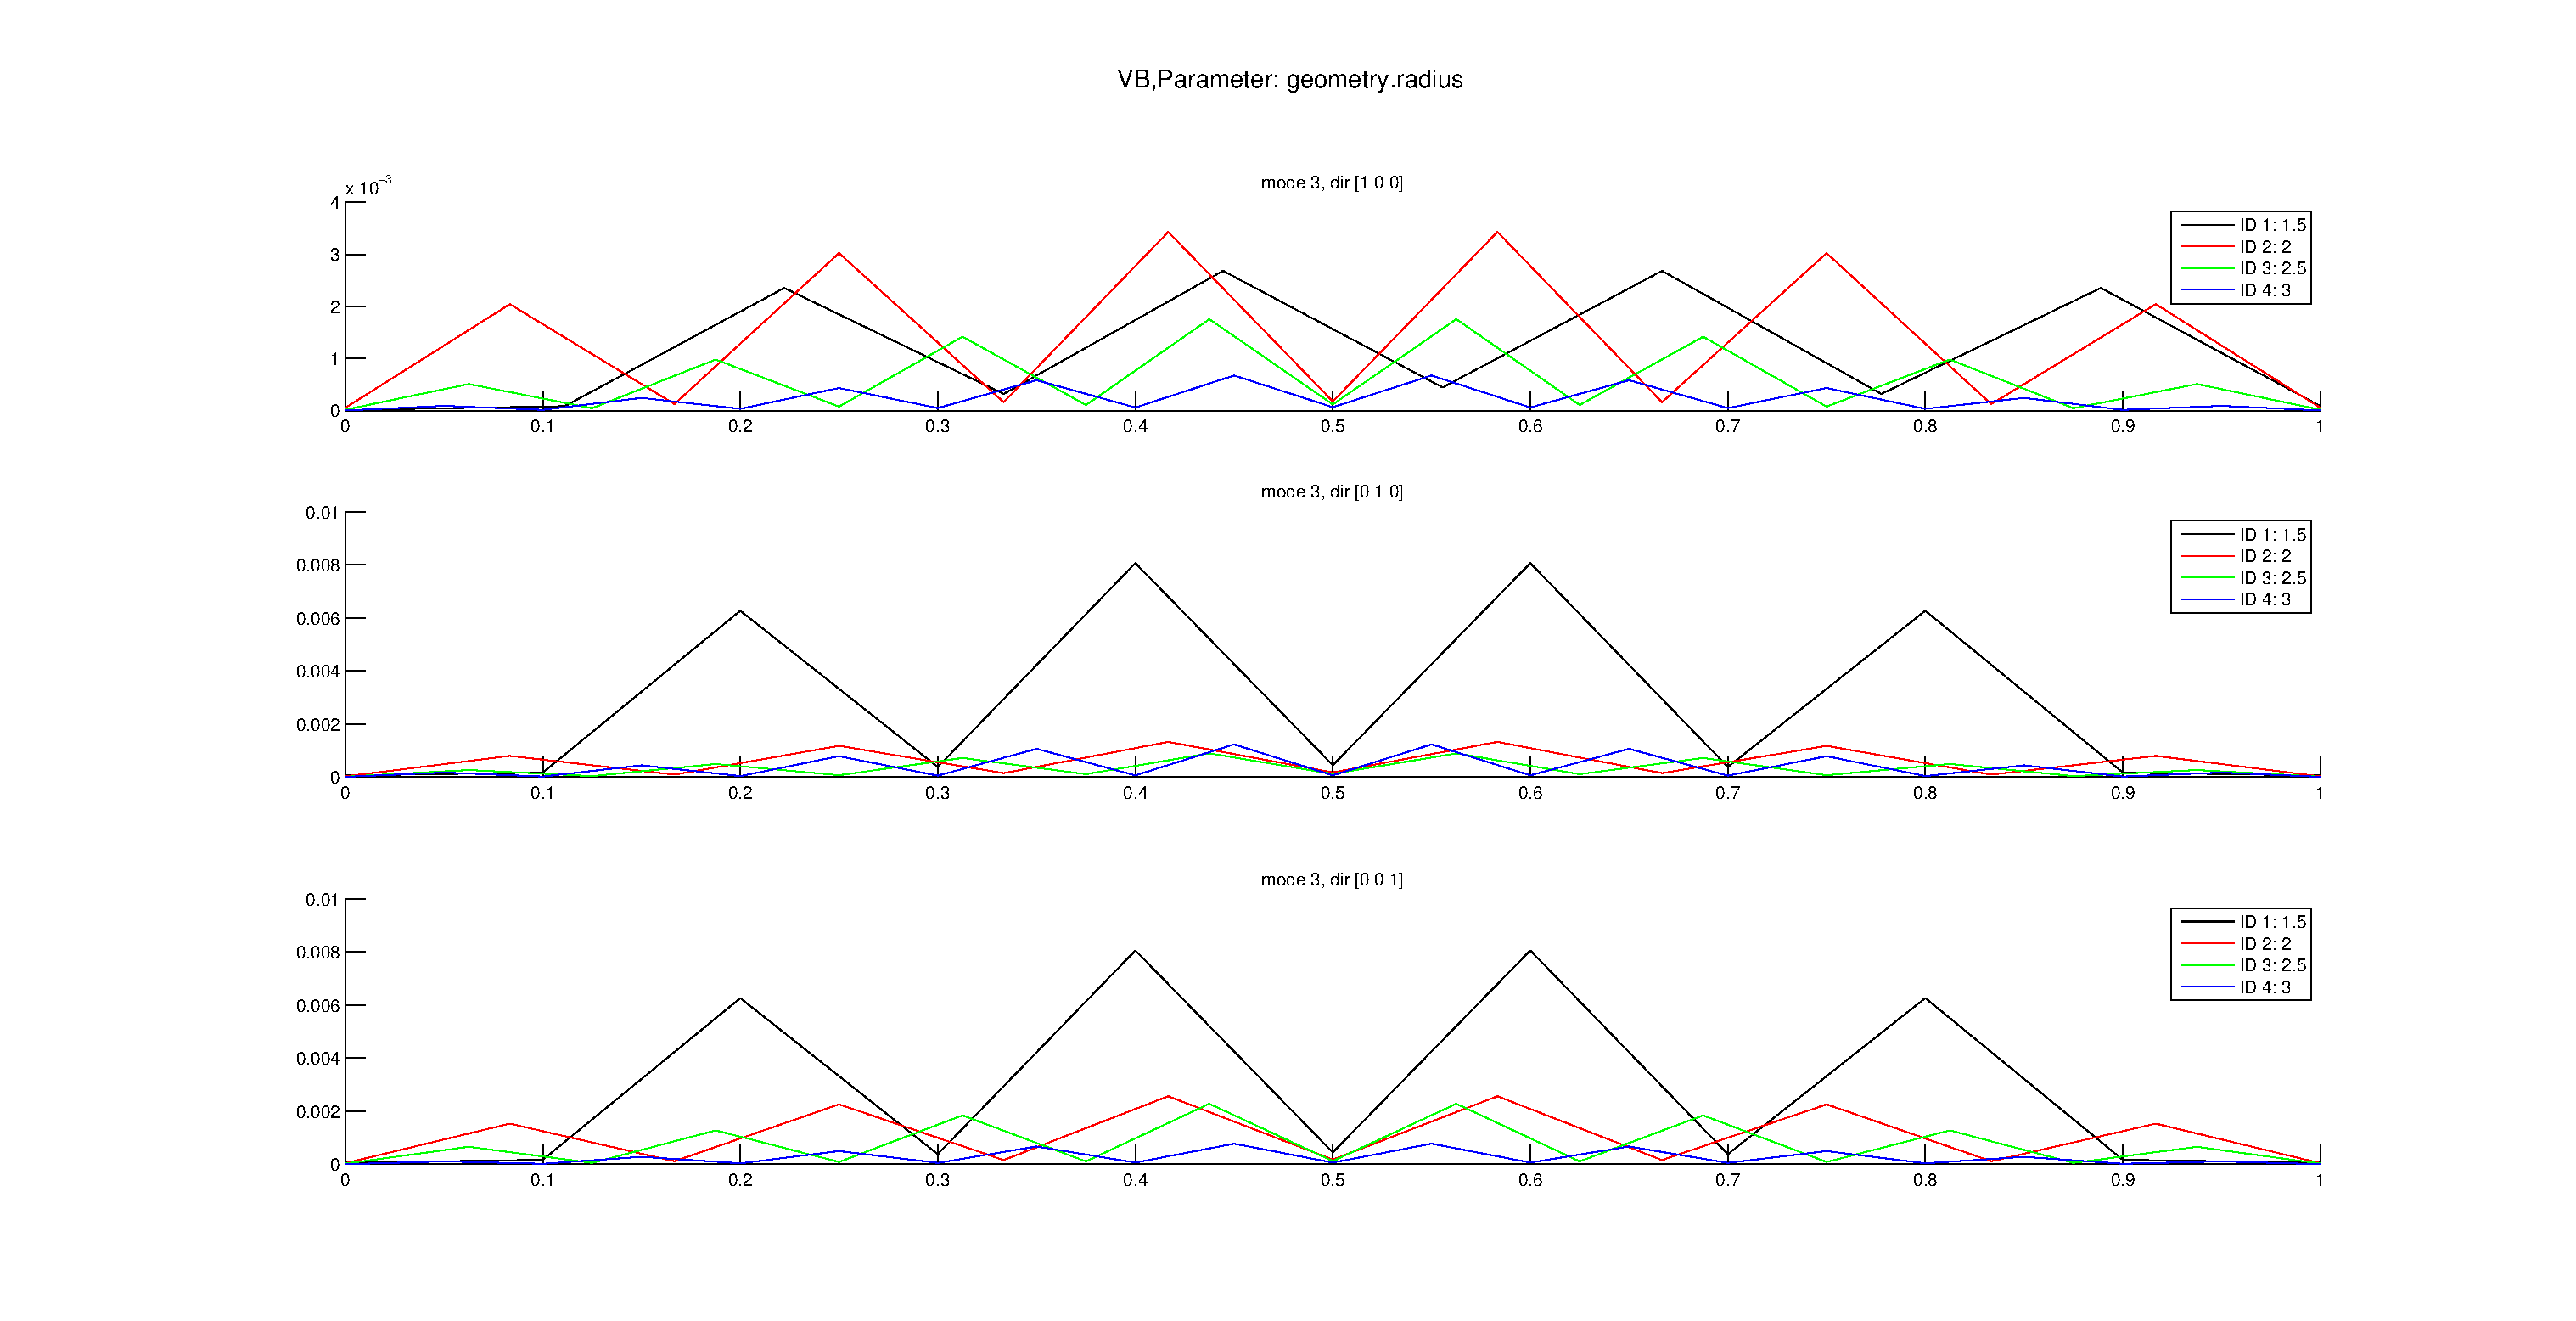
\includegraphics[width=0.9\textwidth]{figures/EVPlot3AxesMod3.eps}
				\caption{Wavefunctions for different radii and directions in the Valence Band Mode 3. The radii are {\it normalized}!}
			\end{figure}
			
			\newpage
			\subsubsection*{3D Wavefunctions for different Voltages}
				\begin{figure}[htbp]
					\centering
					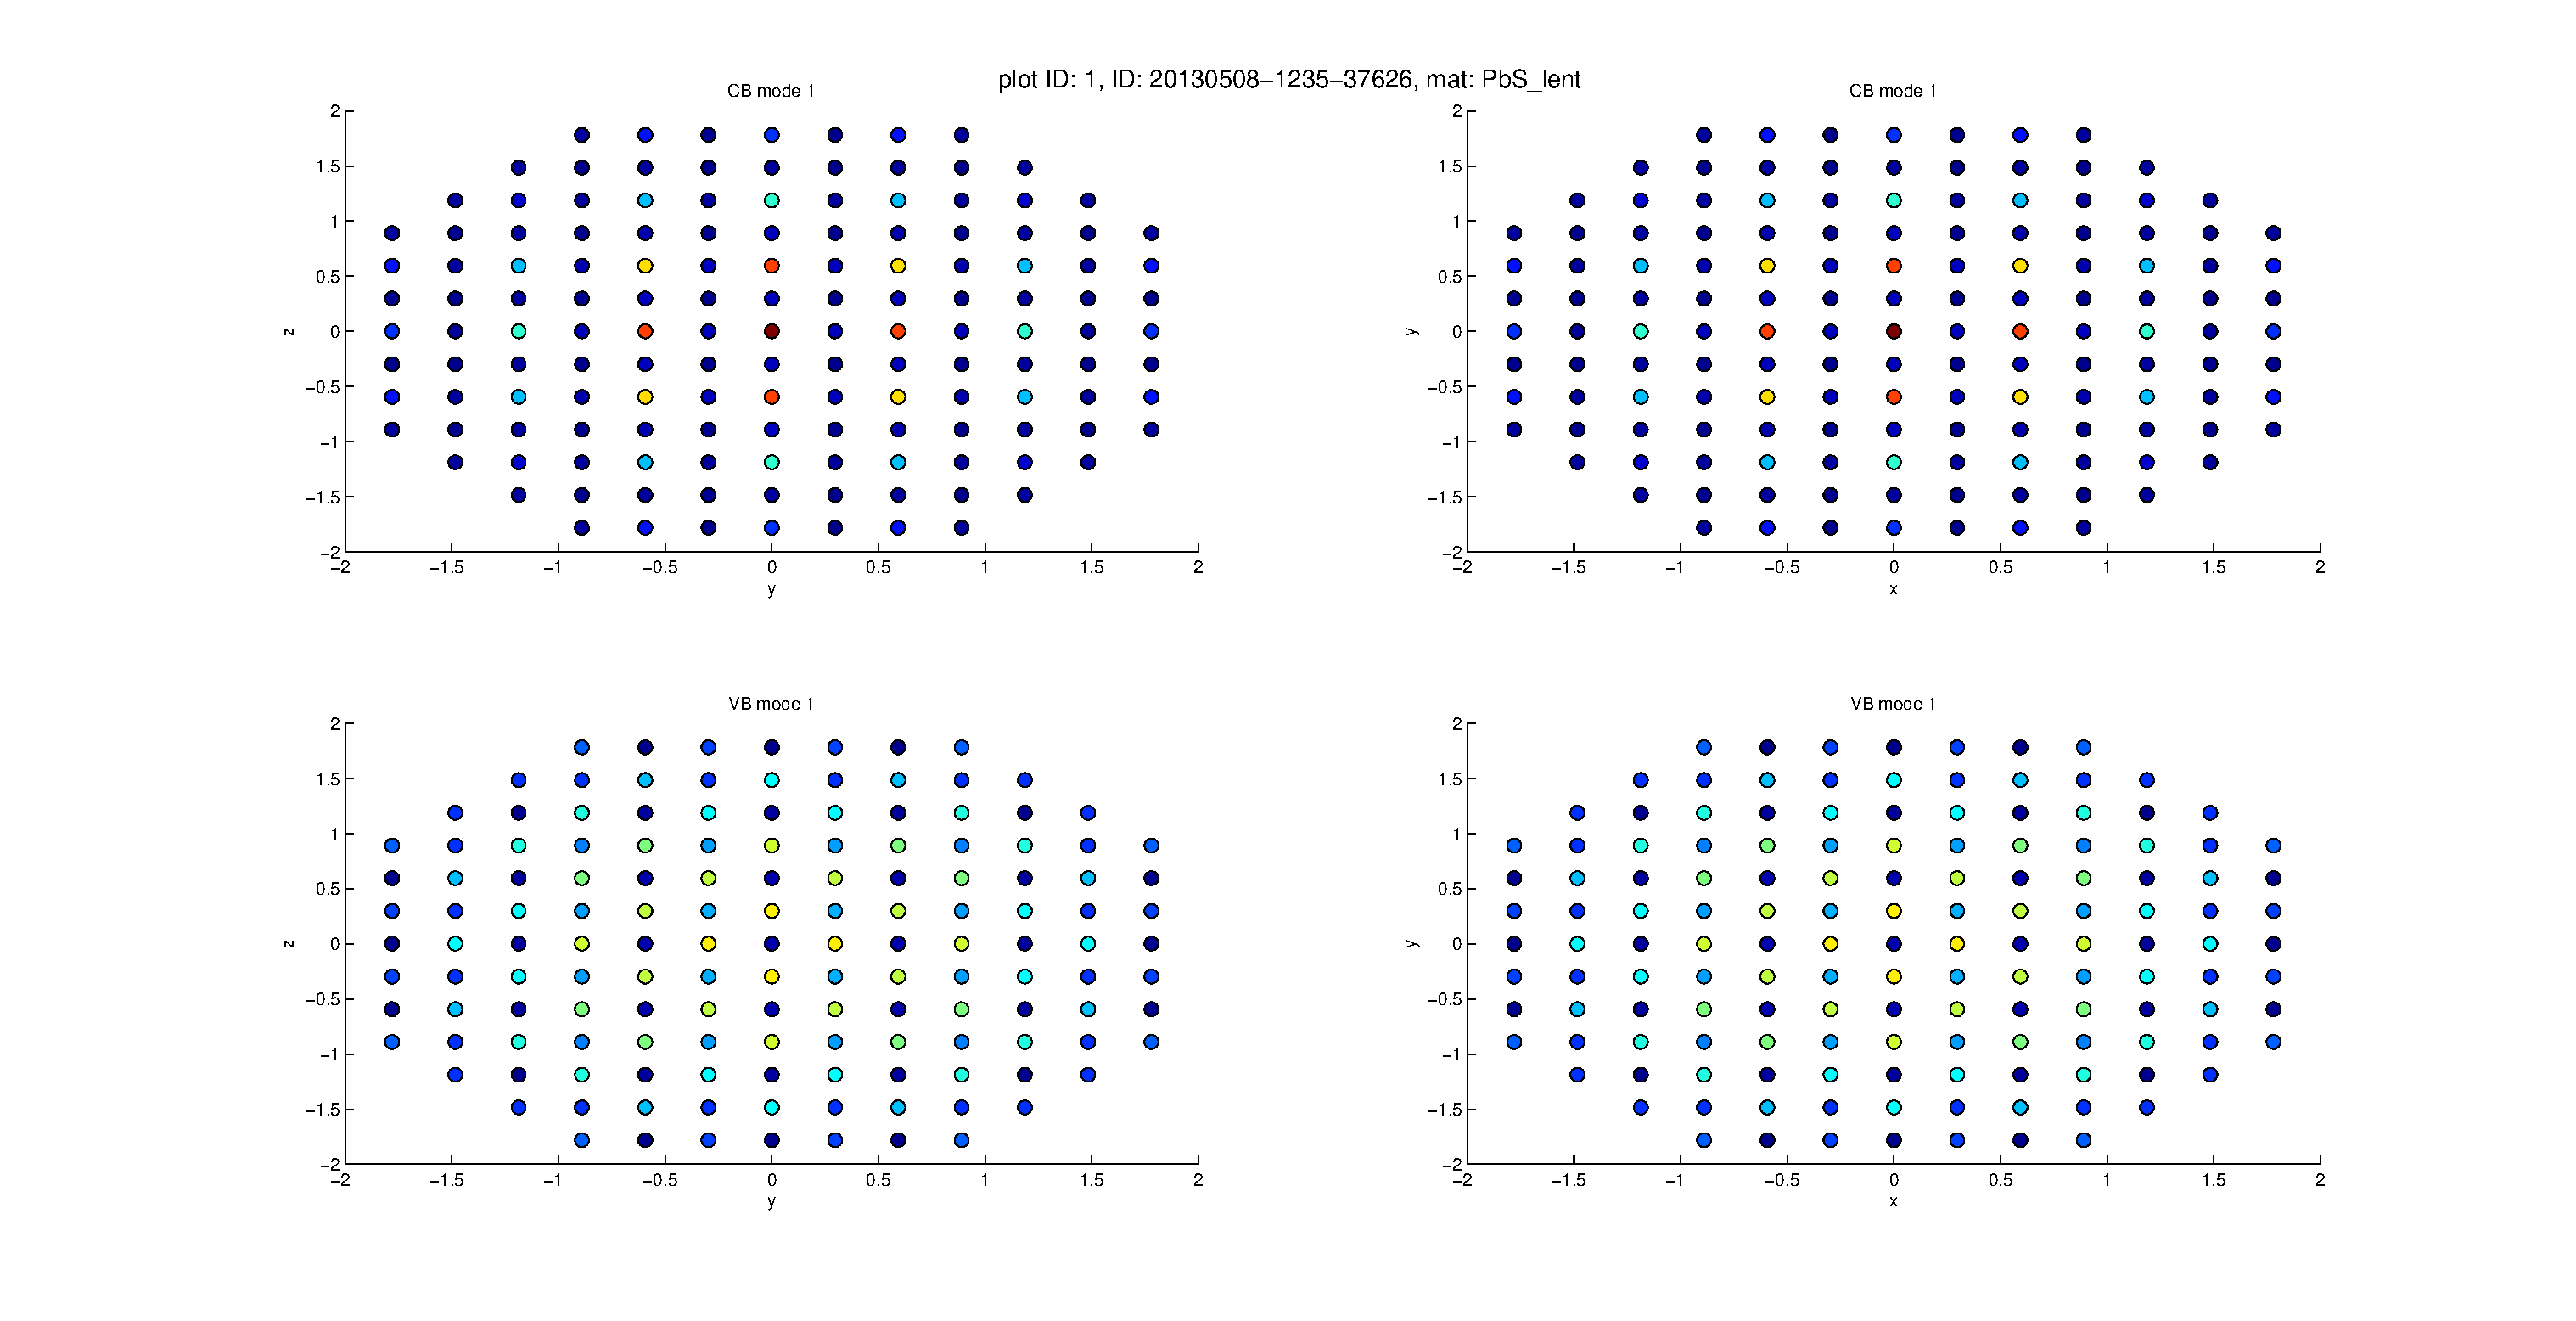
\includegraphics[width=0.9\textwidth]{figures/EVPlot3DVolt1.eps}
					\caption{3D Wavefunctions for 0V of a PbS Quantum Dot with 4 nm  diameter}
				\end{figure}
				\newpage
				\begin{figure}[htbp]
					\centering
					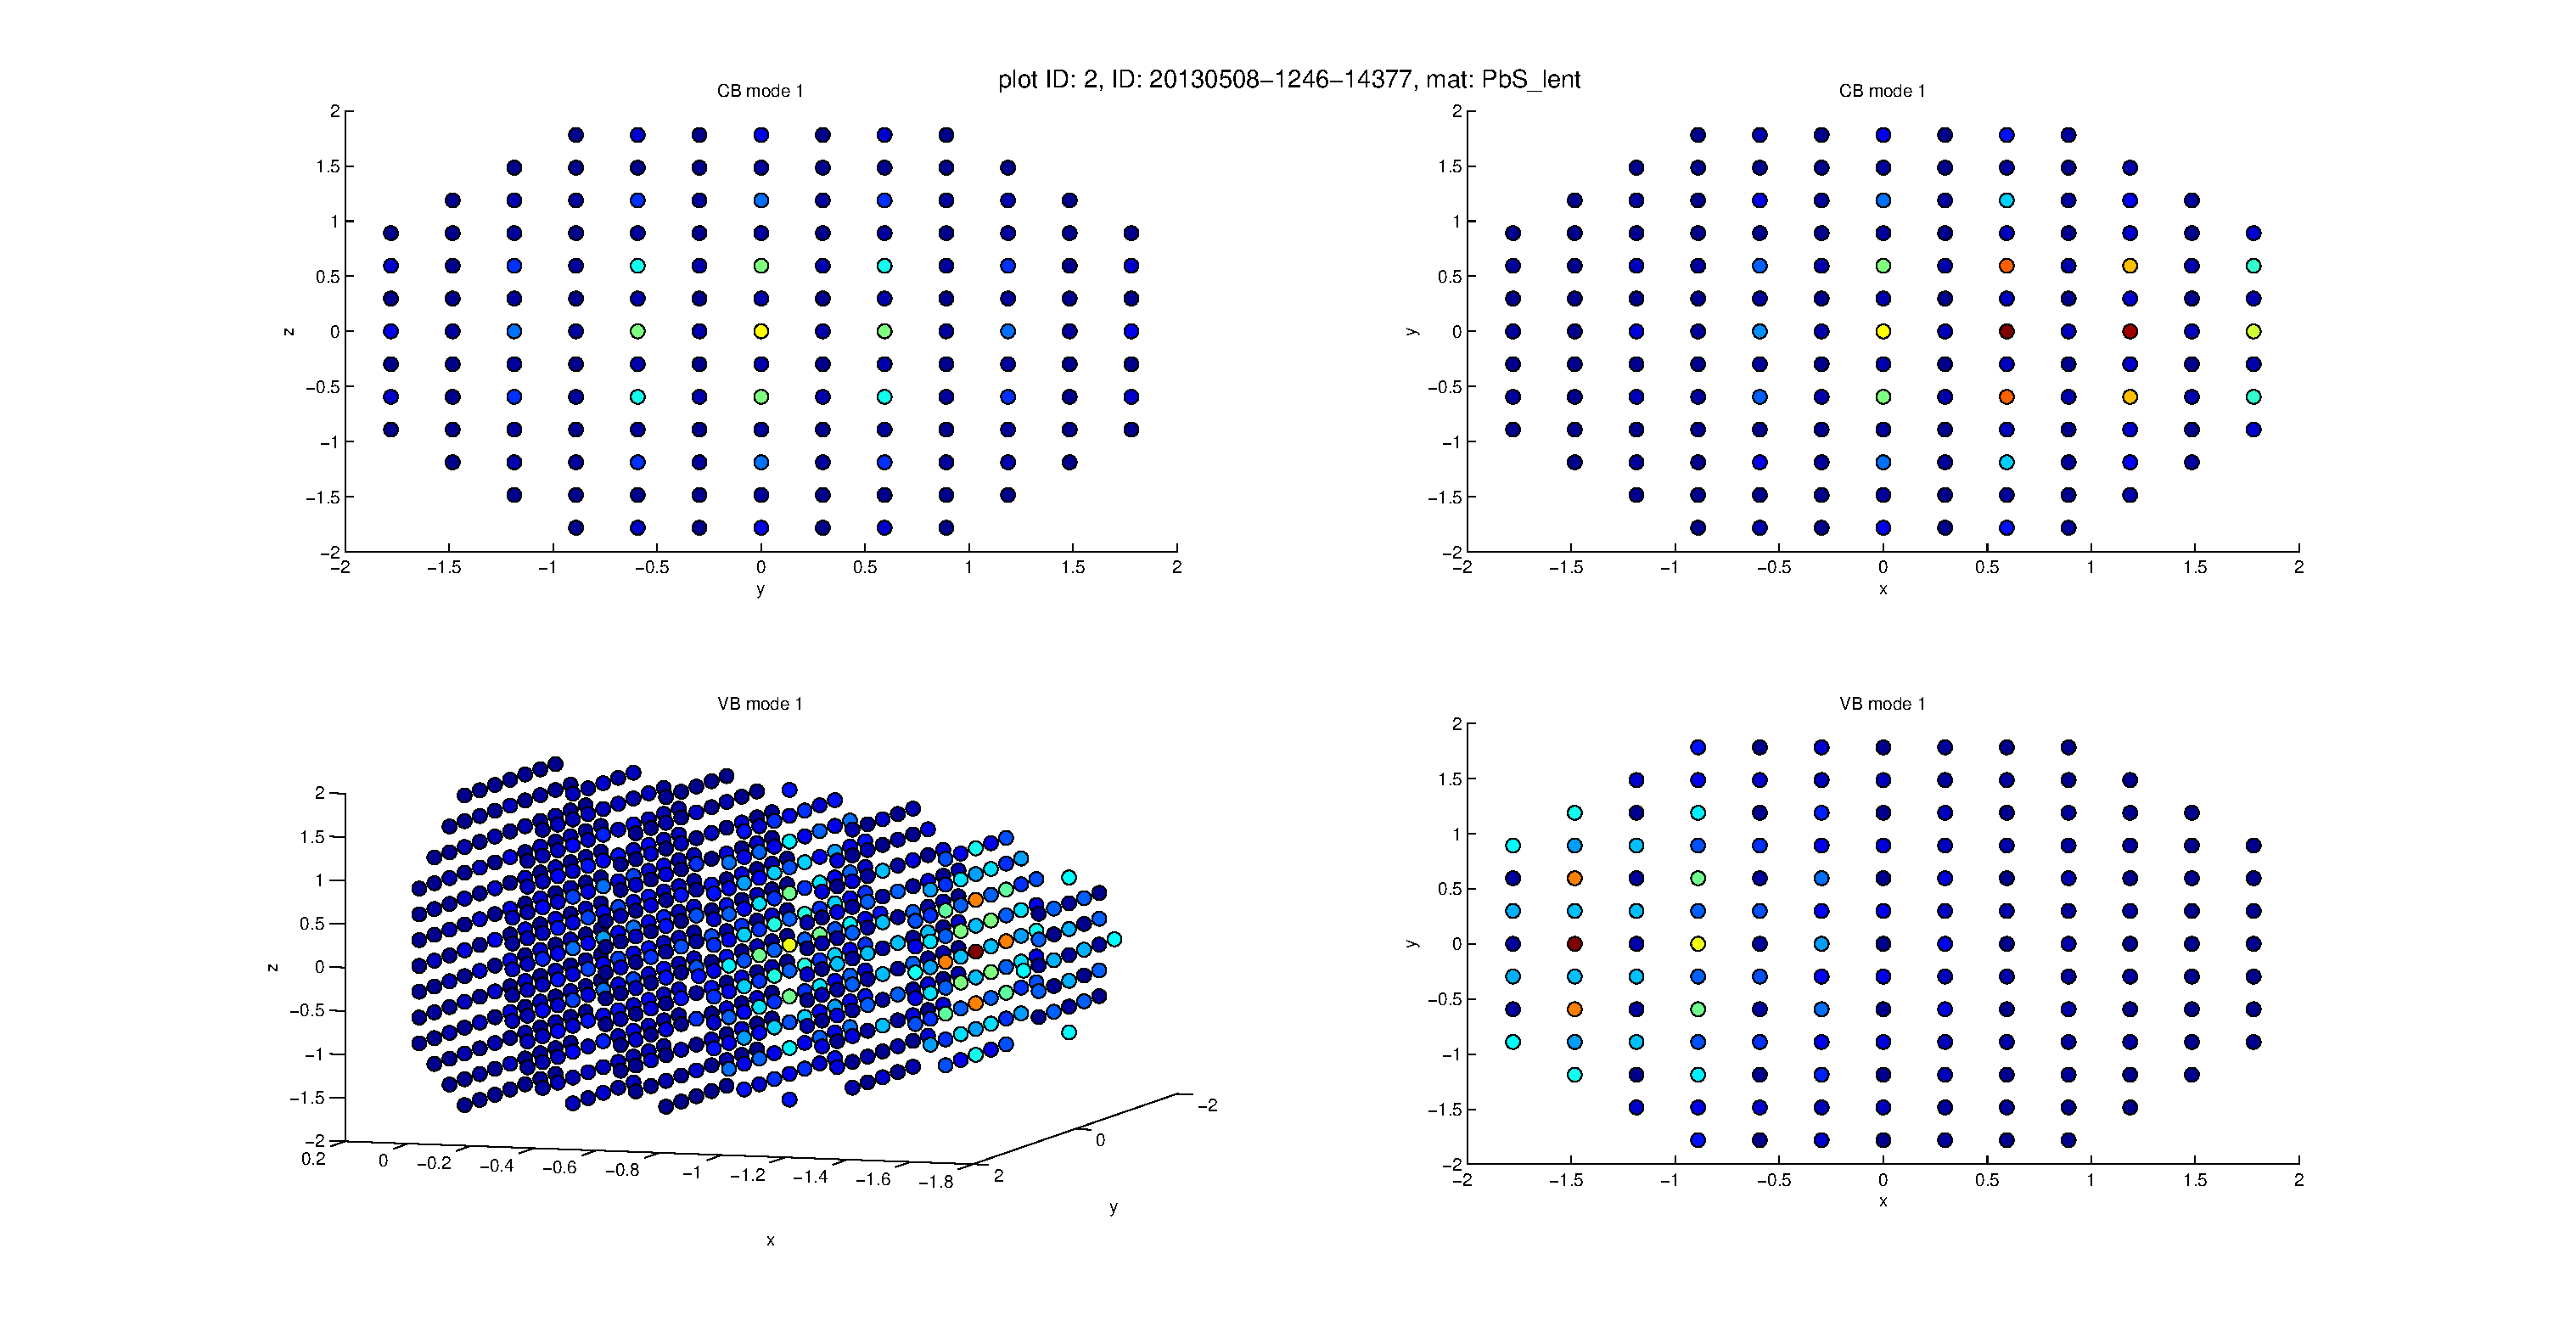
\includegraphics[width=0.9\textwidth]{figures/EVPlot3DVolt6.eps}
					\caption{3D Wavefunctions for 0.5V of a PbS Quantum Dot with 4 nm  diameter}
				\end{figure}

		
		\newpage
		\subsection{Band Gaps}
			\begin{figure}[htbp]
				\centering
				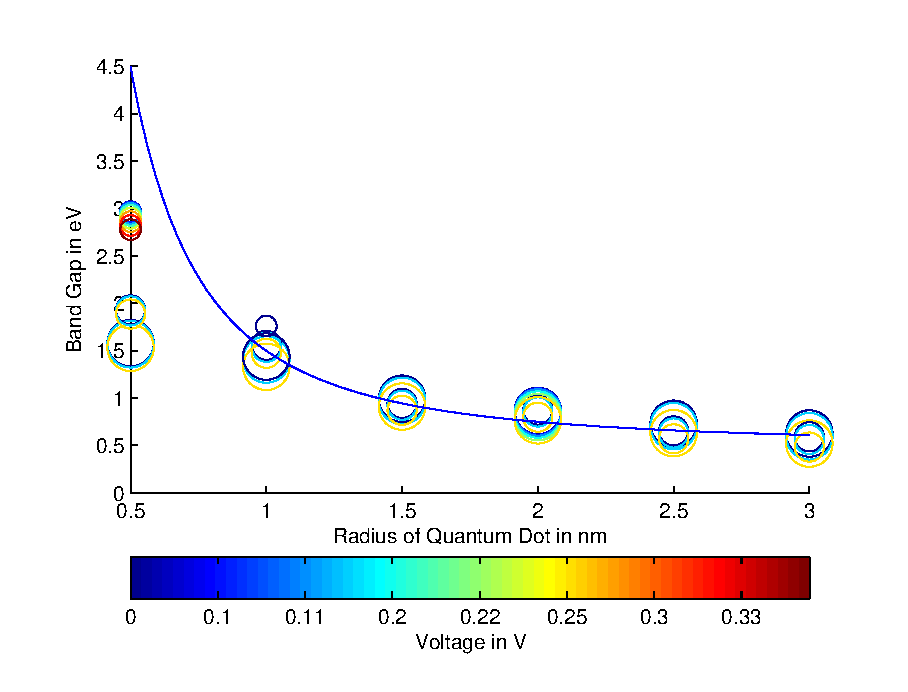
\includegraphics[width=0.6\textwidth]{figures/BandGapAll.eps}
				\caption{Plotting Band Gap against Radius of a Quantum Dot, including applied Voltage and 
								 different materials. Size of the circle indicates the material; from smallest to largest:
								 PbSe\_allan, PbSe\_lent, PbS\_lent. Solid blue line: $1/R^2$ dependence of the Band Gap.}
			\end{figure}
			
			\newpage
			\begin{figure}[htbp]
				\centering
				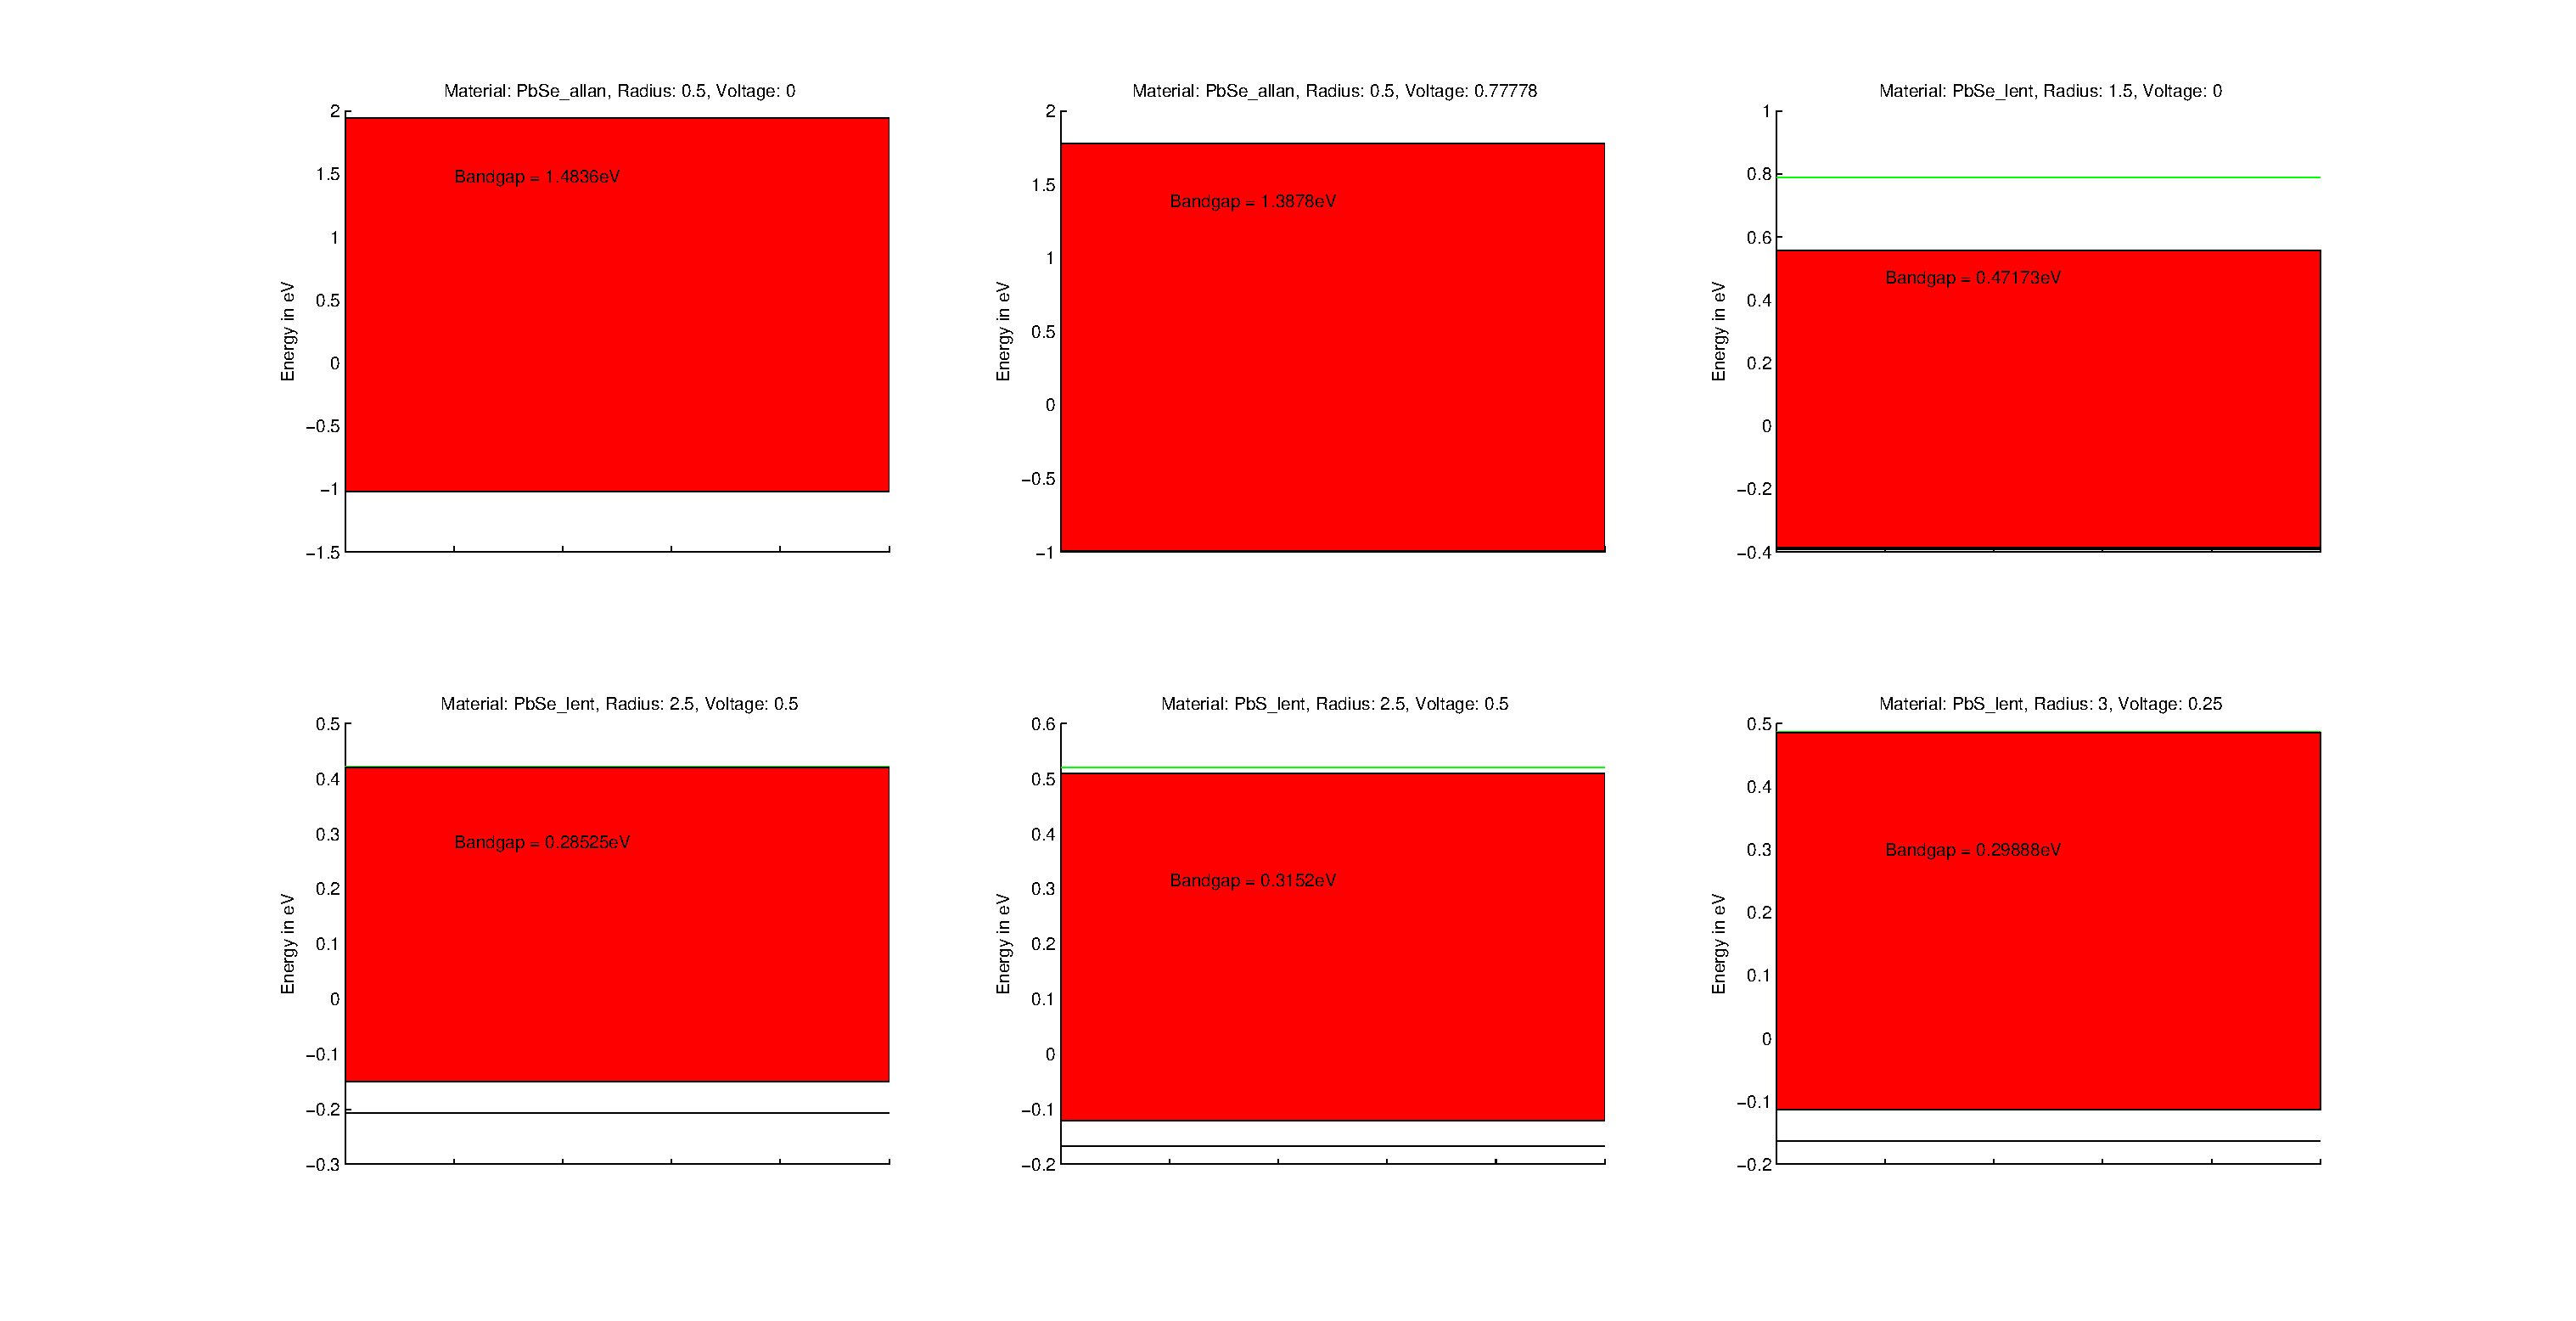
\includegraphics[width=\textwidth]{figures/BandGapsSelected.eps}
				\caption{Green lines: Energy levels in the Conduction Band, Black lines: Energy levels in the Valence Band}
			\end{figure}

\end{document}